\documentclass[a4paper, 11pt]{article}
\usepackage{subfiles}

% PACKAGES
%% document formatting
\usepackage[default]{sourcesanspro}
\usepackage[nottoc,numbib]{tocbibind}

%% languages
\usepackage[ngerman]{babel}
\usepackage{csquotes}

%% hyperlinks
\usepackage{hyperref}
\usepackage{url}

%% graphics
\usepackage{graphicx}
\usepackage{geometry}

%% citation
\usepackage{acronym}
\usepackage[style=ieee]{biblatex}
\usepackage{floatrow}

%% code listings
\usepackage{listings}
\usepackage{xcolor}


% CONFIGURATION
\setlength{\parindent}{0pt}
\hfuzz=10pt 

%% sources
\addbibresource{sources.bib}

%% document link format
\hypersetup{
  colorlinks   = true, %Colours links instead of ugly boxes
  urlcolor     = blue, %Colour for external hyperlinks
  linkcolor    = blue, %Colour of internal links
  citecolor   = red %Colour of citations
}

%% list of figures
\renewcommand{\listoffigures}{\begingroup
\tocsection
\tocfile{\listfigurename}{lof}
\endgroup}

%% listing style
\definecolor{codegreen}{rgb}{0,0.6,0}
\definecolor{codegray}{rgb}{0.5,0.5,0.5}
\definecolor{codepurple}{rgb}{0.58,0,0.82}
\definecolor{backcolour}{rgb}{0.95,0.95,0.92}

\lstdefinestyle{mystyle}{
    backgroundcolor=\color{backcolour},   
    commentstyle=\color{codegreen},
    keywordstyle=\color{magenta},
    numberstyle=\tiny\color{codegray},
    stringstyle=\color{codepurple},
    basicstyle=\ttfamily\footnotesize,
    breakatwhitespace=false,         
    breaklines=true,                 
    captionpos=b,                    
    keepspaces=true,                 
    numbers=left,                    
    numbersep=5pt,                  
    showspaces=false,                
    showstringspaces=false,
    showtabs=false,                  
    tabsize=2
}

\lstset{style=mystyle}

\begin{document}
    \begin{titlepage}
    
\includegraphics[width=0.4\textwidth]{images/HFT_logo}
    \centering
    \vspace{1.5cm}
    {\par \LARGE Erarbeitung und Evaluation einer Laborumgebung zum Thema Webapplication Firewall\par}
    \vspace{1cm}
    {\par \large Bachelor Thesis\par}
    {\par \large im Studiengang Informatik\par}
    \vfill
    \begin{table}[!hbt]
        \centering
        \begin{tabular}{ll}
            Betreuender Dozent:         & Prof. Dr. Jan Seedorf           \\
            Betreuer des Unternehmens:  & Oliver Paukstadt                \\
            Vorgelegt am:               & \today                          \\
            Vorgelegt von:              & Lukas Reinke (Mat. NR. 1001213)
        \end{tabular}\label{tab:info}
    \end{table}
\end{titlepage}
    \section{Abstract}
Hier könnte ihr abstract stehen.

\pagebreak
    \tableofcontents
\pagebreak

\section{Abkürzungsverzeichnis}

\begin{acronym}
    \acro{dmz}[DMZ]{Demilitarisierten Zone}
    \acro{dsgvo}[DSGVO]{Datenschutz-Grundverordnung}
    \acro{http}[HTTP]{Hypertext Transfer Protocol}
    \acro{https}[HTTPS]{Hypertext Transfer Protocol Secure}
    \acro{itsig}[IT-SiG]{IT-Sicherheitsgesetzes}
    \acro{mim}[MITM]{Man-in-the-middle}
    \acro{nat}[NAT]{Network Adress Translation}
    \acro{tls}[TLS]{Transport Layer Security}
    \acro{url}[URL]{Uniefied Resource Locator}
    \acro{rfc}[RFC]{Request for Comments}
    \acrodefplural{rfc}[RFCs]{Requests for Comments}
    \acro{vm}[VM]{Virtuelle Maschine}
    \acrodefplural{vm}[VMs]{Virtuelle Maschinen}
    \acro{waf}[WAF]{Web Application Firewall}
    \acrodefplural{waf}[WAFs]{Web Application Firewalls}
    \acro{xss}[XSS]{Cross Site Scripting}
\end{acronym}

\pagebreak

\listoffigures

\pagebreak

    %chapters
    \section{Einleitung}
    \subsection{Einleitung}
    \label{sec:introuduction}

% WAF relevant weil:
%   markt wachstum
%   DSGVO implizit relevant

Das Feld der \ac{waf} gewinnt aktuell immer mehr an Relevanz.
Dem Markt wird in den nächsten fünf Jahren ein jährliches Wachstum um 19,9 \% auf 14,6 Mrd.\$ vorhergesagt \cite{WebApplicationFirewall}.
Auch Ausarbeitungen zum \textit{Stand der Technik} wie sie zum Beispiel im Deutschen \ac{itsig} und der \ac{dsgvo} gefordert werden, beschreiben eine \ac{waf} als notwendig zur Absicherung einer Webanwendung\cite[3.1.19 Schutz von Webanwendungen]{StandTechnik}.

% was soll vermitttelt werden?
%   was mach WAF
%   wie nutzt man WAF
%   wie greift man WAF an

Diese Bachelor Thesis beschäftigt sich mit der Erarbeitung von Lerneinheiten und einer Laborumgebung anhand derer das Thema \ac{waf} vermittelt werden kann.
Es werden Design beziehungsweise Implementierung einer \ac{waf} betrachtet.
Auch werden Themen vermittelt, die für den Betrieb einer \ac{waf} in einem produktiven Umfeld relevant sind.
Dazu zählen zum Beispiel Deployment und Anpassung einer \ac{waf} an die zu schützende Webanwendung.

%% TODO

\pagebreak
    \subsection{Umfang und Abgrenzung}
    \input{./chapters/01.2_Umfang.tex}
    \pagebreak

    \section{Theoretische Grundlagen}
    \subsection{NAT und Reverse Proxy}
    % NAT (Network Address Translation)
% - Layer 2 & 3 (IP & Port)
% - Internetzugang
% - Funktion: 
%     - Zuordnung von IP-Adressen: n private IPs -> 1 öffentlichen IP.
%     - Adressenspeicherung
%     - Einfachheit des Netzes
% - Sicherheit:
%     - grundlegend
%     - Verbirgt die interne Netzwerkstruktur
%     - keine Verschlüsselung
% 
% Reverse Proxy
% - Layer 5 (HTTP, HTTPS, FTP,\dots)
% - Webanwendungen, CDNs, Schutz interner Netzwerke
% - Funktion:
%     - Abfrageweiterleitung von Clients -> Server
%     - Lastausgleich
%     - Server-Anonymität
%     - Caching
% - Sicherheit:
%     - SSL-Terminierung
%     - Server-Identitäten verbergen
%     - Grundlegende Normalisierungs-Operationen
% 
% Vergleich:
% - NAT: Netzwerkebene <-> Reverse Proxy: Anwendungsebene 
% - Sicherheit: 
%     - NAT: quasi nicht
%     - Reverse Proxy: Verschlüsselung & Normalisierung
%     - Komplexität: Reverse Proxy -> Konfigurationsaufwand
% 
% WAF Nächste stufe
% Konzeptionell Reverse Proxy Modul
    \subsection{HTTP}
    % HTTP (Hypertext Transfer Protocol)
% - Übertragung von Web-Inhalten (Daten für websites)
% - Client-Server-Kommunikation: Clients fragen Webinhalte von Servern an
% - Request-Response Pattern
% - Stateless: Request-Response unabhängig, Kommunikation nicht wiederaufnehmbar
%
% Erweiterungen seit Version 2
% - Multiplexing and Stream Prioritization: 
%     - Mehrere Anfragen und Antworten gleichzeitig
%     - TCP Erweiterung
%     - blocking
% - Push Benachrichtigung:
%     -  Server mehrere Responses auf eine Anfrage
%     - Verbindungen werden nicht sofort geschlossen
% - QUIC 
%     - transport layer Protokoll
%     - nicht mehr TCP basiert
% 
% **Für WAF HTTP v1 Relevant**
% - Grundlegendes HTTP schema verstehen
% 
% **Protokoll**
% Kommunikationsprozess:
% 1. Verbindungsaufbau
%     - Client -> Server
% 2. Anfrage 
%     - Client fragt Daten an oder löst Aktion aus
% 3. Antwort 
%     - Server quittiert Anfrage
%     - eventuell Daten als Antwort
% 4. Verbindung schließen
%     - Server kann eigenständig keine Verbindung zu client mehr herstellen
% 
% Kommunikationsschema:
% 
% HTTP-Request
% - Startzeile:
%     - Methode: 
%         - Aktion (GET, POST, ...)
%         - angelehnt an SQL Datenbank Operationen
%     - Anfrage-URL
%         - Pfad entsprechen UNIX-Path
%         - Prameter (filter) nach `?`
%     - HTTP-Version: 
%         - Version der folgenden Kommunikation
% - Header
% - Body
% 
% HTTP-Response
% - Statuszeile:
%     - Status Code: 
%         - Numerischer Code
%         - Status der Verarbeitung (200:OK, 400 User Fehler, 500: Server Fehler, ...)
%     - Status-Text: 
%         - Beschreibung des Status code
% - Header
% - Body
% 
% HTTP-Header:
% - zusätzliche Informationen (Host, User-Agent, Content-Type, ..)
% - Enthalten Metadaten über die Anfrage oder den Client/Server.
% 
% HTTP-Body
% - Optional
% - Daten

Das Hypertext Transfer Protokoll (HTTP) ist ein Protokoll in der Internet-Kommunikation, dass zur übertagung diverser Daten unterschiedlicher Datentypen genutzt werden kann. Sein Haupt-Einsatzgebiet ist die Datenübertragung zwischen Webseiten und Clients.
Seit der Einführung in 1991 wurde es in mehreren RFCs erweitert und ist inzwischen in version drei.\\

In seiner aktuellen Form kann es Gebrauch von TCP-Sitzungen machen um Verbindungen über längere Zeit aufrecht zu halten und fortgeschrittenere Kommunikation, wie push Nachrichten, zu erlauben. Außerdem kann TCP-Pipelining genutzt werden um die parallele Abarbeitung von Anfragen zu ermöglichen und nicht auf die \textit{Acknowledge}-Nachrichten von TCP warten zu müssen.
Um seine Grundfunktion zu erläutern wird in diesem Kapitel die statuslose Kommunikation, definiert in Version 1.0 die mit einem unmittelbaren Anfrage-Antwort Muster arbeitet, beschrieben.
Hierin initiiert ein Client mit einer Anfrage Nachricht \footnote{Im folgenden werden HTTP-Anfrage und das Englische HTTP-request synonym verwendet} eine Verbindung, die von einem Server verarbeitet und mit einer Antwort-Nachricht beantwortet wird. Darauf wird die Verbindung geschlossen.
Dem Sever ist es nun nicht mehr möglich dem Client weitere Daten zu senden, ohne das der Client eine weitere Anfrage-Nachricht schickt.

\paragraph{HTTP-Nachrichten}
Die Grundlegende Einheit einer \ac{http}-Kommunikation wird als \textit{Nachricht} bezeichnet.
Da \ac{http} ein Klartext-Protokoll ist, werden diese in menschenlesbarer Form als Text übertragen.
Eine Nachricht besteht aus einer \textit{Start-Zeile}, die die Nachricht entweder als Anfrage oder Antwort identifiziert. In diesen beiden Fällen hat die Zeile jeweils einen untersiedlichen Aufbau:

\begin{description}
     \item[Request-Zeile:] Ein HTTP-Request ist durch eine \textit{Request-Zeile} identifiziert. Diese ist in drei Teile Aufgeteilt.
     \begin{description}
          \item[Die HTTP-Methode:] beschreibt die   
     \end{description}
     \item[Status-Zeile:] 
\end{description}


\pagebreak    
    \subsection{OWASP Top-Ten}
    % Standard für die Sicherheit von Webanwendungen 
% wichtigsten Sicherheitsrisiken für Webanwendungen
% Regelmäßig upgedatet um den gegenwärtigen stand darzustellen
% 
% - Broken Access Control
%     - Fehler die zu unerlaubten Privilegien führe
%     - Least-privilege Prinzip
%     - Privilege escalation
% - Verschlüsselungsfehler
%     - veraltete Protokolle
%     - neue Schwachstellen
% - Injection
%     - SQL, noSQL, LDAP, ...
% -  unsicheres Design
%     - Der Applikation inherente Fehler
% - Fehlkonfigurationen
% - Anfällige und veraltete Komponenten
% - Identifizierung- und Authentifizierungsfehler
%     - Fehler in Zugangskontrolle
% -  Fehler bei der Software- und Datenintegrität
%     - Fehler bei der Prüfung von Daten-Validität(Updates, Externe Pakete,...)
% - Fehler beim Logging
% - Server-Side Request Forgery
    \subsection{Web Application Firewall}
    % - Sicherheits-Applikation/ Spezielle Firewall
% - Gefordert in diversen Compliance Richtlinien
% - Fokus auf web-Protokolle
%     - auf TCP/IP Layer 5
%     - HTTP, HTTPS, FTP
% - Traffic Analyse in Tiefe (Request & Response)
%     - HTTP (kapitel 5.2) beschreibt diverse Angriffswege
%     - Erkennung anhand von Regeln
%         - Black- vs. whitelisting
%         - Vordefiniertes Regelwerk
\label{chap:waf-theory}

Mit dem Namen \ac{waf} wird eine Sicherheits-Anwendung beschrieben, die in der Lage ist den Datenverkehr zu und von einer Webanwendung zu analysieren und auf Sicherheitskritische Inhalte zu überprüfen. 
Eine \ac{waf} ist hierbei in der Lage gefährliche Inhalte nicht nur zu blockieren, sondern anfragen auch so zu verändern, dass sie unschädlich sind und trotzdem verarbeitet werden können.
Im Gegensatz zu einer \textit{klassischen} Firewall, die auf den Schichten 3 und 4 des OSI/ISO Schichten-Modells arbeitet, ist eine \ac{waf} in der Lage passierenden Datenverkehr auf der Anwendungsschicht (Schicht 7) zu analysieren. 
Hierbei liegt der Fokus hauptsächlich auf dem \ac{http}. Es ist jedoch auch möglich andere, im Kontext von Webanwendungen genutzte Protokolle wie FTP zu analysieren.
Um des gesamten Inhalt der zu analysierenden Nachrichten sehen zu können (Deep Packet Inspection) kann eine \ac{waf} Protokolle zur Sicherstellung von Vertraulichkeit und Integrität (SSL/TLS) terminieren.
\\
Es gibt mehrere kommerzielle Hersteller aber auch Opern-Source Entwickler die \acp{waf} zur Verfügung stellen.
Diese Angebote können auf eine vielzahl von Wegen logisch vor einer Webanwendung positioniert werden.
Während große Hosting- und Serveranbieter wie Cloudflare or Microsoft azure es ermöglichen mittels wenigen kicks eine \ac{waf} vor die bei ihnen untergebrachten webserver zu installieren, können die Angebote anderer, eigenständiger \acp{waf} auf unterschiedliche Methoden betrieben werden:
\begin{enumerate}
     \item Als physischer Server in einem Rechenzentrum
     \item Als Eigenständige virtuelle Maschine innerhalb der eingenen Virtualisierungsumgebung
     \item Als Einheit in einer Containervirtualisierungsumgebung
     \item Als Modul oder Addon einer Webserver-Anwendung (NGINX/Apache webserver)
\end{enumerate}

Daraus ergeben sich zwei gängige Deployment Szenarien.

\begin{itemize}
     \item \textit{On premise Deployment} bei dem sich die \ac{waf} neben den zu schützenden Anwendungen im gleichen Netzwerk befindet
     \item \textit{Cloud WAF} wo die \ac{waf} von einem Drittanbieter zur Verfügung Gestellt wird und mittels IP-Whitelisting sichergestellt werden muss, dass ein zugriff auf die Webanwendung nur durch die \ac{waf} erfolgen kann.
\end{itemize}
Der Betrieb einer \ac{waf} erfordert die Anpassung an die zu schützende Anwendung. Es muss eine Konfiguration sichergestellt werden, dass die Funktion einer Webanwendung nicht beeinträchtigt ist ohne dabei die schützenden Funktion der \ac{waf} einzuschränken.

Um abgrenzen zu können welche Inhalte für Lerninhalte in Frage kommen und abzuschätzen was in der vorgegeben Zeit vermittelt werden kann wird im folgenden Kapitel eine \ac{waf} detailliert beschrieben.

\subsubsection{Verarbeitung einer Anfrage}
\paragraph{Request Parsing}
% - SSL Termination
% - HTTP/HTTPS Parsing
% - Nachsichten Felder extrahieren
% - Anfragen Normalisierung
% - Überführen in ein standardisiertes Format
% - Gegen diverse evasion techniken
%     - null byte
%     - self-referencing directories
%     - path traversals
%     - URL encoding

\begin{figure}[!hbt]
    \centering
    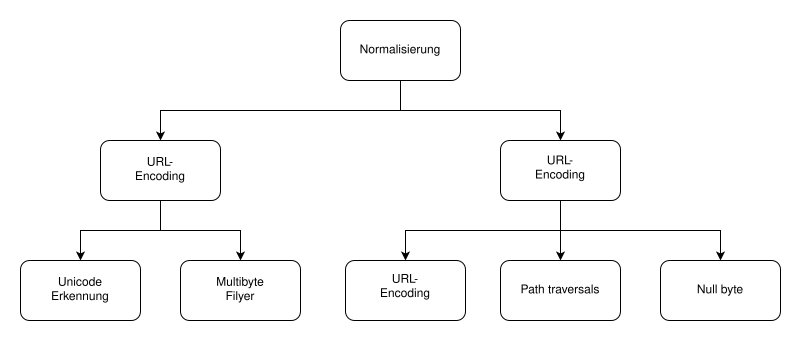
\includegraphics[width=0.9\textwidth]{./images/Normalisierung.png}
    \caption{Normalisierungs-Schritte}
    \label{fig:norming}
\end{figure}


\paragraph{Muster-Abgleich gegen Regeln}
% - Abgleichen gegen Feature Datenbank
% - Jeder Parameter gegen jede regex
%     - Rechenaufwand
%         - optimierte regex-Engines
%         - Tree pruning
%             - Gefahr durch ungewollte pass on Szenarien
% - Whitelisting
%     - Features deaktivieren die web app-Funktion einschränken
% - Blacklisting
%     - Default Regelwerk
% - Auch Signatur-basierte WAFs
%     - komplexere Erkennung

\paragraph{Logging}
% - Jeder Schritt wird protokolliert
%     - Compliance
%         - Erfiltrierte Daten
%         - betroffene Nutzer
%     - Nachvollziehbarkeit von Fehlern
% - Log analyse
%     - Hauptarbeit eines WAF-Consultants

\paragraph{Weiteres Vorgehen}
% - Request Ablehnen
%     - Werden schädliche Daten erkannt
% - Request modifizieren
%     - Ablehnen bei schädlichen Inhalten nicht notwendig
%     - request kann umgeschrieben werden
%         - Abschnitte entfernen
%         - Abschnitte Escapeen
% - unmodofiziertes weiterleiten
% 
% - aus normalisierter form HTTP-Request erstellen
% - an server übergeben

\subsubsection{Erweiterte Funktionen}
\paragraph{Lernen von Regeln aus vorhergegangenem Datenverkehr}
\paragraph{KI-Features}
\subsubsection{Deployment einer WAF}
\paragraph{Postitionierung einer WAF}
\paragraph{Betrieb einer WAF}
\subsubsection{Schwächen und Nachteile einer WAF}

    \pagebreak

    \section{Design der Lernumgebung}
    \subsection{Zu übermittelnde Inhalte}
    \label{chap:inhalte}
    Dieses Kapitel beinhaltet die Beschreibung der Laborumgebung deren Erstellung eines der Hauptziele dieser Thesis ist.
Es werden zuerst Abwägungen zu den Inhalten, die übermittelt werden sollen, angestellt.
Des Weiteren werden Produkte evaluiert die für die Realisierung der Laborumgebung genutzt werden können und deren Nutzung in der Laborumgebung beschrieben.
Es wird sowohl eine \ac{waf} als auch eine Anwendung benötigt, die zu schützende Schwachstellen aufweist.
Final werden die erstellten lerneinheiten beschrieben und Abwägungen angestellt wie die Lerneinheiten die erarbeiteten Leerinhalte übermitteln können.

\subsection{Zielsetzungen und grundlegende Überlegungen}
\label{sec:learnings-metha}

%Wird eine \ac{waf} als Schutz einer Webanwendung eingesetzt unterscheidenden sich die Aufgaben die für den Betrieb ausgeführt werden müssen deutlich von den Inhalten, die 
% ToDo Waf wird in Vorlesung vorgestellt
% ToDO Zeitvorgabe
Der Fokus der Lerneinheiten soll auf der Funktion einer \ac{waf} liegen.
Die Lerneinheiten sind nicht geeignet um das Aufgabenfeld von \ac{waf}-Consultants zu vermitteln.
Der Fokus liegt auf dem Erkennen, Verstehen und abwehren von Cyber-Angriffen.
Im Betrieb einer \ac{waf} wird das hierfür notwendige Regelwerk mit den Produkten vorkonfiguriert ausgeliefert.
Die Aufgaben in diesem Fall sind die Reaktion und Adaption der \ac{waf} auf entstehende Fehler um die Nutzung der zu schütztenden Webseite ohne Funktions-Einschränkungen zu ermöglichen.

In der Laborumgebung sollen diese vorkonfigurierten Regeln von den Lernenden erarbeitet werden.
Die Entstehende Konfiguration ist höchst spezialisiert und kann in einem realen Szenario nicht ansatzweise Sicherheitsvorteile erbringen.
Die bei einer Produktiven-\ac{waf} mitgelieferten Regelwerke werden von Mathematikern oder Theoretischen Informatikern erstellt und sind deutlich Allgemeingültiger als diejenigen die in dieser Laborumgebung erarbeitet werden.\\

Die Lerneinheiten sind angelegt begleitend zu theoretischem Unterricht durchgeführt zu werden.
Parallel zu der Durchführung sollen die Lernenden das Wissen erhalten welches in den Grundlagen-Kapiteln (Kapitel \ref{sec:theoretical-foundations}) beschrieben ist.
Die Laborumgebung ist nicht dafür ausgelegt dies theoretischen Grundlagen zu vermitteln und stützt sich zu Teilen auf dieses Wissen.
Die Lerneinheit soll in einer Vorlesung mit 4 SWS innerhalb dreier Wochen durchführbar sein.
Das Heißt es werden pro Lerneinheit 3 bis 5 Stunden Zeitaufwand angesetzt.

Die Laborumgebung besteht aus drei, aufeinander aufbauenden Lerneinheiten.
In einem erste Schritt soll, nachdem sich mit dem Aufbau der Laborumgebung vertraut gemacht wird, die generelle Position einer \ac{waf} im Netzwerkverkehr beschrieben werden.
Es sollen unkompliziert zugängliche Inhalte des \ac{http}-Protokolls analysiert werden um den generellen Aufbau einer einer Regel und die schritte der Verarbeitung in einer \ac{waf} zu Verstehen.\\

Die Zweite Lerneinheit beschäftigt sich mit grundlegenden Angriffen die von einer \ac{waf} abgefangen werden können.
Hierfür werden einige grundlegende Schwachstellen herangezogen die sowohl in der Realität auftreten als auch ohne Vorkenntnisse mit Sicherheitslücken in Webanwendung verständlich sind.
Die benötigten Vorkenntnisse sollen nur im Bereich der Software-Entwicklung und der Erstellung von Webseiten sowie einem Grundverständnis des \ac{http}-Protokolls liegen.
Anhand dieser Kenntnisse und der Beschreibung von Schwachstellen in der zu schütztenden Webanwendung soll ich ein Verständnis der Angriffsvektoren erarbeitet werden und ein Regelwerk erstellt werden, das diese abdeckt und die Ausnutzung vereitelt.

Um neben dem Regelwerk auch einen Einblick in den betrieb einer \ac{waf} zu vermittel fokussiert sich die dritte Lerneinheit darauf mit einer \ac{waf} im alltäglichen Betrieb zu arbeiten.
Hier sollen die Lernenden mit einer Fehlerhaften \ac{waf}-Regel Konfrontiert werden, die das rechtmäßige Funktionieren der Webanwendung  hinter der \ac{waf} beschränkt.
Sie sollen diese Regel analysieren, mit den Folgen für die Netzwerkkommunikation beschäftigen und die Regeln adaptieren, sodas die Funktion der Webseite wiederhergestellt werden kann.
Des Weiteren soll die dritte Lerneinheit sich mit Techniken der Filter-evasion beschäftigen.
Hier sollen sich die Lernenden mit Techniken auseinandersetzen, die genutzt werden können um zu verhinder, dass ein Regulärer Ausdruck einen schädlichen Inhalt als solchen erkennt.
Solche Techniken werden in realen Angriffsszenarien an einem Filter vorbei Angriffe zu ermöglicht.
Eine \ac{waf} bietet auch für derartige Angriffe Verteidigungen.
    \subsection{Technische Umsetzung}
    \subsubsection{Evaluation verfügbarer Produkte}
\label{chap:produkt-eval}
\paragraph{Auswahl der \ac{WAF}-Anwendung}

\paragraph{Verwundbare Anwendungen}

\subsubsection{Labor-Umgebung}

% 1. Anforderungen an die Lernumgebung
% 2. Überlegungen zur gestaltung einheiltichen Deployments
% 2.1. Docker
%       - einheitlich
%       - Netzwerke
%       - Probleme mit croscompatibility (Windows)
% 2.2. VM (vortiele und Probleme)
% 3. beschreibung der Container
% 3.1. Juicesop
% 3.2. WAF
% 3.3. Python contaienr mit test script

Die in Kapitel \ref{chap:inhalte} beschriebenen Inhalte sollen in einem Praxisnahen Umfeld vermittelt werden.
Dazu kommt nach den Abwägungen aus Kapitel \ref{chap:produkt-eval}, die Waf-Applikation ModSecurity zum Einsatz.
Die zu diesem Zweck vorgesehene Laborumgebung muss einige Kriterien erfüllen:
\begin{description}
    \item[Einheitliches Deployment:]  Der Ausgangspunkt der Lerneinheiten muss reproduzierbar und wiederholbar sein. Bei wiederholten Durchführungen der Übungen soll es einfach sein den Lernenden ohne zusätzlichen Manuellen Konfigurationsaufwand eine Laborumgebung zu übergeben.
    \item[Modifizierbarketit der Anwendungen:] Um in den Lerneinheiten grundlegende Techniken zu übermitteln, ist es notwendig Basis-Funktionen entfernen zu können. Und die 
    \item[Bekannte Basis-Technologien:]
    \item[Komplexe Netzwerkumgebungen:]
\end{description}

\begin{figure}[!hbt]
    \centering
    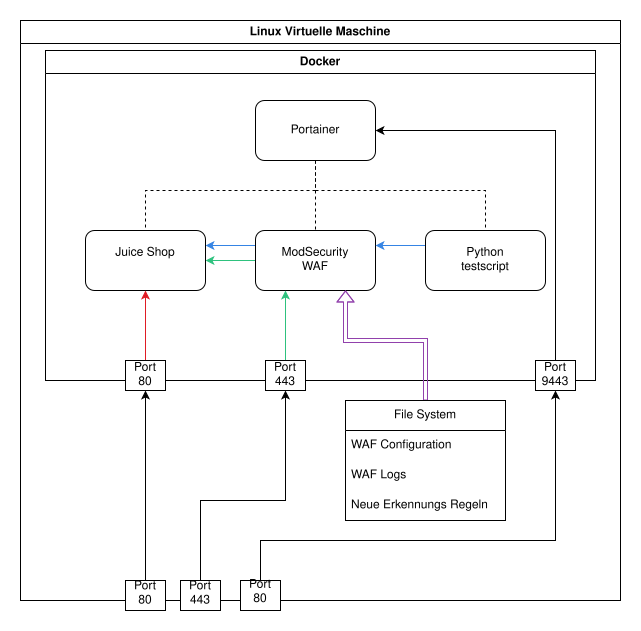
\includegraphics[width=0.9\textwidth]{./images/lab-setup.png}
    \caption{Aufbau der Laborumgebung}
    \label{fig:lab}
\end{figure}


    \subsection{Lerneinheiten}
    Die in diesem Kapitel beschriebenen Lerneinheiten machen in der praktischen Arbeit einen zentralen zentralen Bestandteil dieser Thesis aus.Sie ähneln sich in Aufbau und Durchführung, beschäftigen sich jedoch mit unterschiedlichen Aspekten einer \ac{waf}:
Eine Aufgabe in einer Lerneinheit beginnt immer mit einigen Worten zu dem Thema mit dem sich die Lernenden beschäftigen sollen, gefolgt von einer Referenz auf eine Challenge aus dem Juice Shop die mit der \ac{waf} abgesichert werden soll.

In diesem Kapitel wird beschrieben welche Überlegungen in die Konzeption der Lerneinheit geflossen sind.
Mit welchem Oberthema sich die jeweiligen Lerneinheiten beschäftigen, nach welchen Kriterien die Challenges des Juice Shops ausgewählt wurden und wie die Challenges gelöst werden können.

\subsubsection{Teil 1: Erster Kontakt zu einer WAF}
\label{sec:learning-unit-1-meta}

In der ersten Lerneinheit sollen sich die Lernenden mit der Laborumgebung vertraut machen.
Erst sollen die Lernenden die Laborumgebung auf ihren Geräten einrichten und sich versichern, dass sie Zugriff auf alle Services der Umgebung haben.
Dann gilt es ein Verständnis aufzubauen wie der Fluss einer \ac{http}-Anfrage durch die Netzwerke der Umgebung erfolgt.
Den Lernenden sollte vor Beginn der Lerneinheit bekannt sein wie eine \ac{waf} in der Theorie vor eine Webanwendung platziert werden kann.\\

Die eigentlichen Aufgabenstellungen zu der hier beschrieben Lerneinheit sind in Anhang \ref{sec:learning-unit-1} zu finden.\\

\paragraph{Einrichtung der Laborumgebung}\ \\

In der ersten Aufgabe (Anhang \ref{sec:learning-unit-1-preparations}) der Lerneinheit sollen die Lernenden die Laborumgebung installieren.
Hierfür muss die die \ac{vm} der Laborumgebung bereit gestellt werden.
Die weiteren Anwendungen, die im Zuge der Durchführung benötigt werden, werden in der Aufgabenstellung genannt und die Konfiguration erläutert.
Die Aufgabe besteht aus einer detailliert bebilderten Anleitung zum Aufsetzen der Laborumgebung.
Die Bestandteile sind:

\begin{enumerate}
    \item Installation der \ac{vm}
    \item Konfiguration eines virtuellen \textit{Host-Only} Netzwerkadapters um vom Host Betriebssystem auf die \ac{waf}-Laborumgebung zugreifen zu können.
    \item Abrufen der Verfügbaren Webanwendungen
    \item Verbinden mit der SSH-Schnittstelle um die \ac{waf} Konfiguration bearbeiten zu können.
\end{enumerate}

Die Anleitung ist mit dem Fokus auf einige notwendige und empfohlene Technologien verfasst.
Es wird nur die gängigste Methode beschrieben die Laborumgebung aufzusetzen: Windows und VirtualBox.
Es wird jedoch auch auf einer konzeptionellen Ebene beschrieben, was zu tun ist.
Lernende, die andere als die beschrieben Technologien nutzen möchten, können dies tun, dies ist in der Konzeption der Laborumgebung berücksichtigt, wird in der Anleitung aber nicht genauer beschrieben.
Lernende die sich dafür entscheiden müssen auftretende Probleme mit den von ihnen gewählten Technologien eigenständig und ohne Hilfe der Anleitung lösen.

Nach Abschluss der Aufgabe müssen die Lernenden in der Lage sein, die Laborumgebung zu nutzen um weitere Aufgaben zu lösen.
Die Lernenden müssen sich nur in geringem Maße neues Wissen erarbeiten, da die Anleitung sehr eng geführt ist.

\paragraph{Erste Arbeit mit der WAF}\ \\

In dieser Aufgabe in der sich die Lernenden das erste Mal mit \ac{waf}-Regeln beschäftigen.
Für den Einstieg soll sich zuerst mit der Syntax der \textit{ModSecurity} Regeln anhand einfacher Beispiele beschäftigt werden.
Hierfür werden zwei Challenges des \textit{Juice Shops} herangezogen deren Lösungen ohne größere Probleme nachvollziehbar sind.
In der Ersten dieser Aufgaben soll ein Pfad unzugänglich gemacht werden, auf dem sensitive Informationen preisgegeben werden.
Die hierfür notwendige Regeln ist verhältnismäßig unkompliziert und kann beispielsweise wie Folgt aussehen:

\begin{verbatim}
SecRule REQUEST_URI "@streq /ftp/acquisitions.md" \
    "id:1, \
    msg:'Stop access to critical /ftp/aquisitions.md', \
    deny, \
    status:403"
\end{verbatim}

Der zweite Teil der Aufgabe erfordert es, den Inhalt eines \ac{http}-Bodies zu parsen und zu analysieren.
Die zugehörige Challenge im \textit{Juice Shop} weist eine Schwachstelle auf, in der Parameter im Backend nicht auf Gültigkeit geprüft werden.
Dadurch können ungültig Daten an den Webserver übergeben werden, die dort gespeichert und von dort an Nutzer übergeben werden.
Der Parameter \textit{rating}, der in einem JSON-Objekt im \ac{http}-Request Body transportiert wird soll nur die Werte 1 bis 5 annehmen können.

Der schädliche Parameter kann auf unterschiedlichen Wegen erkannt werden.
Zwei Beispiele wären:\\

\begin{itemize}
    \item Mithilfe eines regulären Ausdrucks ($[\land 1-5]$):
    \begin{verbatim}
    SecRule REQUEST_HEADERS:Content-Type "application/json" \
        "phase:2, id:3, t:none, t:lowercase, \
        log, ctl:requestBodyProcessor=JSON" \
        chain, \
        msg:'JSON parameter rating found in request body'"
    
        SecRule REQUEST_BODY:rating "@rx [^1-5]" \
            "id:4, phase:2, \
            deny, log, status:403"
    \end{verbatim}

    \item Mithilfe von Vergleichsoperationen (\textit{@gt 5} und \textit{@lt 1}):
    \begin{verbatim}
    SecRule REQUEST_HEADERS:Content-Type "application/json" \
        "phase:2, id:3, t:none, t:lowercase, \
        log, ctl:requestBodyProcessor=JSON" \
        chain, \
        msg:'JSON parameter rating found in request body'"
        
        SecRule ARGS:rating "@gt 5" \
            "id:4, phase:2, \
            deny, log, status:403"
    
        SecRule ARGS:rating "@lt 1" \
            "id:5, phase:2, \
            deny, log, status:403"
    \end{verbatim}
\end{itemize}

Diese Challenges sollen den Lernenden grundlegende Konzepte zum Aufbau einer \textit{ModSecurity} Regel beibringen:
\begin{itemize}
    \item Den grundlegenden Aufbau nach der Struktur
    \begin{verbatim}
        SecRule VARIABLE [OPERATOR] [TRANSFORMATIONS,ACTIONS]
    \end{verbatim}
    in der erst das Ziel der Operation (VARIABLE), dann die Matching-Operation (OPERATOR) und dann das Verfahren nach dem \textit{Match} (TRANSFORMATIONS,ACTIONS) beschrieben werden.
    \item Das Prinzip des \textit{Multi Stage Processing}: Nicht die ganze \ac{http}-Nachricht steht zur gleichen Zeit zur Verfügung. Der Zugriff auf ein JSON-Body Element kann, wie in dem Beispiel oben, also erst nach vorherigem Parsing betrachtet werden.
\end{itemize}

Die beiden oben beschrieben Aufgaben sind gedacht, um die \ac{waf} kennen zu lernen.
Sie bilden jedoch kein Verhalten ab das in einer \ac{waf}-Regel einer produktiven \ac{waf} verwendet werden würde:
Die Regeln sind viel zu detailliert und auf einen spezifischen Fall ausgerichtet.

\subsubsection{Teil 2: Grundlegende Angriffe}
\label{sec:learning-unit-2-meta}

Nachdem sich in der ersten Lerneinheit mit der Laborumgebung, der \ac{waf} und ihrer Funktion vertraut gemacht wurde, kann der Fokus in dieser zweiten Lerneinheit auf Angriffsszenarien gelegt werden.
Die Lernenden beschäftigen sich exemplarisch mit zwei Angriffsszenarien, die in der aktuellen IT-Sicherheit und Verteidigung von Webanwendungen relevant sind.\\

Die Aufgabenstellungen zu der hier beschreiben Lerneinheit sind in Anhang \ref{sec:learning-unit-2} zu finden.

\paragraph{SQL Injections}\ \\
Die SQL-Injection ist eine Angriffstechnik bei der Nutzereingaben direkt und ungefiltert an eine SQL-Datenbank im Backend weitergegeben werden.
Dies kann zu unvorhergesehenen Nebeneffekten wie Befehlsausführung auf dem Server und Daten-Exhilaration führen.
Nach \textit{OWASP-Top-Ten} gehören SQL Injections zu den zehn schwerwiegendsten Schwachstellen, die in Webanwendungen zu finden sind.

Die Funktion und Verteidigung gegen SQL Injection Angriffe sollen Lernenden in dieser Aufgabe erarbeiten.
Zuerst soll sich mit einer spezifischen Sicherheitslücke beschäftigt werden und diese mit einer eigenständigen \ac{waf}-Regel mitigiert werden.
In einem zweiten Schritt wird einen SQL-Injection generell betrachtet.
Hierfür sollen die Lernenden die Gemeinsamkeiten von zwei \textit{Juice Shop} Challenges herausarbeiten und beide Schwachstellen mit einer Regel mitigieren.

Die erste Teilaufgabe beschäftigt sich mit einem SQL Login-Bypass.
Zum Abgleich, ob ein Nutzer existiert und das Passwort gültig ist, wird im Backend die SQL-Datenbank genutzt.
Ein Angreifer kann in dieser \textit{Juice Shop} Challenge an den Nutzernamen einen Vergleich in SQL Syntax anhängen und somit einen gültigen Login erzwingen ohne das Passwort eines Nutzers zu kennen.

Um diesen Angriff erkennen zu können, sollen sich die Lernenden auf escape syntax fokussieren, mit deren Hilfe ein SQL-Befehl beendet werden kann, um danach eigene Befehle auszuführen.

Zwei Beispiele könnten wie Folgt aussehen:

\begin{verbatim}
SecRule ARGS:email "@rx ^['].*--" \ 
    "id:6, phase:2, \
    deny,log,status:401"

SecRule ARGS:email "@rx ==\w*--" \
    "id:7, phase:2, \
    deny,log,status:401"
\end{verbatim}

In beiden Fällen wird nach dem Beginn eines SQL Kommentars gesucht.
Die beiden dargestellten Möglichkeiten suchen vor dem Kommentar jedoch nach unterschiedlichen Angriffsmustern.
Im ersten Beispiel werden Hochkommata gemacht, die in einer Mailadresse nicht vertreten sein sollten.
Im zweiten Fall wird nach einem Vergleich ($==$) gesucht, der zwar theoretisch in einem nicht bösartigen Szenario vorkommen könnte, jedoch eher unwahrscheinlich ist und keine Einschränkung für Nutzer darstellen würde.
Der \ac{http}-Error-Code der in diesen Beispielen zurückgegeben wird unterscheidet sich zu denen, die in den Regeln aus Aufgabe 1 (siehe Kapitel \ref{sec:learning-unit-1-meta}) vorkommen.
Dies liegt an der unterschiedlichen Situation:
In diesem Beispiel handelt es sich um Fehlende Autorisierung eine Anfrage zu machen:
Der status code 401 (Unauthorized) wird gewählt.
Im vorherigen Beispiel ist der Zugang zu der Resource generell verboten: der status code 403 (Forbidden) wird gewählt.

Im zweiten Teil der Aufgabe soll sich nun auf das generelle filtern von SQL-Syntax fokussiert werden.
Die beiden Challenges die die Lernenden analysieren sollen weisen SQL-Injection Schwachstellen im HTTP-Body auf.
Damit die Lernenden keine Regeln schreiben können, die sich nur auf einen spezifischen Fall beschränkt sollen die Lernenden eine Regel für beide Challenges schreiben.

Ein Lösungsvorschlag für das generelle Erkennen einer SQL-INjection Attacke kann sein die sql keywords zu erkennen wie in dem folgenden regulären Ausdruck nachvollziehbar ist.

\begin{verbatim}
\s*(select|union|update|delete|insert|drop|--|or|and|alter|exec
|create|script|table|from|where|join|having|cast)\s*
\end{verbatim}

Beim schreiben der Regel müssen die Lernenden darauf achten, dass die Regel keine unvorhergesehenen Nebeneffekte hat.
Wird beispielsweise nur nach dem substring \verb|and| gefiltert, könnte ein Nutzer mit dem Namen \textit{Andy} Probleme bekommen die Webanwendung zu nutzen.\\


Ist die Aufgabe abgeschlossen sollen die Lernenden ein Verständnis dafür haben wie eine SQL-Injection Funktioniert.
Außerdem sollen sie durch das lösen von Problemen und betrachten der Logs herausgefunden haben, dass ein regulärer Ausdruck dessen Folgen nicht bedacht wurde Probleme bei der regulären Nutzung der Webanwendung hervorrufen kann.

\paragraph{Cross Site Scripting (XSS)}\ \\

Neben der \textit{SQL-Injection} nutzen Angreifer häufig sogenannte \ac{xss} Schwachstellen in Webanwendungen aus.
Bei einem \ac{xss} ist es einem Angreifer möglich HTML und Java Scrip Code an die Webanwendungen zu übergeben sodass dieser von der Anwendung nicht als Text interpretiert wird sonder als Code Ausgeführt bzw. dargestellt wird.

In diesem Teil der Lerneinheit sollen sich die Lernenden mit der Funktion einer \ac{xss} Schwachstelle vertraut machen und daraus ableiten, wie ein solcher Angriff erkannt und verhindert werden kann.
Des weiteren besitzen Browser Funktionen die das Ausnutzen eines \ac{xss} erschweren.
Diese werden können in einem HTTP request durch das Setzen eines bestimmten Headers oder dem erstellen einer \textit{Content Security Policy} die festlegt von welchen Quellen Daten nachgeladen werden dürfen.
Dies kann auch durch die \ac{waf} erfolgen.
An diesem Beispiel ist es auch möglich das Umschreiben eines \ac{http}-Request durch die \ac{waf} zu übermitteln.

Im ersten Teil der Aufgabe sollen die Lernenden eine \ac{waf}-Regel schreiben die in eingehendem Traffic ein HTML-Tag und javascript erkennt und Blockiert.
Es existieren mehrere Möglichkeiten einen solchen Angriff zu erkennen und abzuwehren.
Anhand der öffnenden und schließenden HTML-Tags oder dem \textit{javascript} Tag.
Im folgenden beispiel ist eine Möglichkeit dies anhand der HTML \textit{script Tags} zu tun dargestellt:

\begin{verbatim}
    SecRule REQUEST_HEADERS:Content-Type "application/json \
        [...]
        SecRule ARGS: "@rx <script[^>]*>.*</script>|<[^>]+>" \
        [...]
\end{verbatim}

Für eine allgemeine Lösungen nicht hinreichende, jedoch in dem spezifischen Fall der Übung gültige Lösung wäre das erkennen des javascript codes.
Das Hierfür zum Testen genutzte \textit{javascript:alert} ist austauschbar und würde keinen zuverlässigen Schutz sorgen.

Der Zweite Teil der Aufgabe beschäftigt sich mit dem mit dem setzen des \textit{X-XSS-Protection} Headers.
Hierfür muss in einer Regel ausgehender Netzwerkverkehr erkannt werden.
Anstatt diesen zu blockieren kann der Header gesetzt werde, wie im Folgenden Beispiel zu sehen ist:

\begin{verbatim}
SecRule RESPONSE_HEADERS:@streq 200 \
   "id:10, phase:3, nolog, pass,\
   hdrOut: Header set X-XSS-Protection '1; mode=block'"
\end{verbatim}

Die Lernenden sollen nach Abschluss dieser Lerneinheit ein Verständnis für die Funktion eines \ac{xss} haben.
Außerdem soll ein Bewusstsein für die Funktion der \ac{xss}-Protection Header bestehen, die einen wichtigen ersten Verteidigungsschritt gegen diese Angriffe darstellen.
Neben dem Verständnis für den Angriff wird auch die Fähigkeit einer \ac{waf} den Netzwerkverkehr nicht nur zu bloc sonder auch umzuschreiben vermittelt.

\subsubsection{Teil3: Nutzung einer WAF in produktivem Umfeld}
\label{sec:learning-unit-3-meta}

Die dritte Lerneinheit soll einen Fokus auf der Arbeit mit einer \ac{waf} in produktivem Umfeld Legen.
Die Lernenden sollen mit den Logdateien arbeiten um den Fehler in einer \ac{waf}-Regel zu finden.
Außerdem ist vorgesehen, dass sich die Lernende mit Techniken der \textit{Filter evasion} beschäftigen, die ein Angreifer Nutzen könnte um nicht von den regulären Ausdrücken einer \ac{waf} erkannt zu werden.\\

Im Rahmen der Thesis war es aus Zeitlichen gründen diese dritte Lerneinheit zu realisieren.

    \pagebreak

    \section{Evaluation}
    \subsection{Evaluation mit Probanden}
    Um einschätzen zu können wie die Lerneinheiten in der Lehre eingesetzt werden könne wird eine Evaluation durchgeführt.
Wie viel Zeit wird für die Durchführung der Übungen benötigt?
Welche Vorkenntnisse sind notwendig um die Übungen erfolgreich durchführen zu können?
Welches wissen erwerben die Lernenden in der Laborumgebung?

Bevor die Laborumgebung begonnen wird, soll eine Selbsteinschätzung durchgeführt werden in der die Kenntnisse zu bestimmten Technologien abgefragt werden, die in der Laborumgebung relevant sind.
Die Teilnehmer sollen auf einer Skala von 1 bis 6 ihre Fähigkeiten in den folgenden Technologien bewerten:

\begin{itemize}
    \item Linux
    \item Virtuelle Maschinen
    \item Containervirtualisierungsumgebung Docker
    \item Softwareentwicklung
    \item Reguläre Ausdrücke
    \item HTTP auf Protokollebene
    \item SQL-Syntax
    \item Sicherheitslücken in Webanwendung
    \item Web Application Firewall
\end{itemize}

Nach der Selbsteinschätzung werden die Lerneinheiten durchgeführt.
Die Probanden sollen die Lerneinheiten eigenständig bearbeiten damit das Umfeld möglich nah an dem geplanten Einsatzgebiet der Laborumgebung ist.



\subsection{Evaluation mit Probanden}

Die Evaluation 

% Zeit
% Scheitern 
% da war noch was drittes



    \subsection{Überlegungen zur Bewertung}
    Als Teil der Thesis wird sich mit der Frage beschäftigt, wie eine Bewertung der Ergebnisse, die die Lernenden in der Laborumgebung erarbeiten, erfolgen kann.
Kann erkannt werden ob lernende Lösungen untereinander austauschen?
Es wird auch die Möglichkeit untersucht ob es möglich ist, die Laborumgebung so dynamisch zu generieren, dass die Laborumgebungen für jeden Lernenden einzigartig gestaltet ist.
Dies ließe sich beispielsweise durch dynamisch generierte Netzwerk-Topologien erreichen.
Einen weitere Möglichkeit wäre, jedem Lernenden unterschiedliche zu schützenden Challenges des \textit{Juice Shops} zuzuweisen.
Beide Ansätze stellen sich in der Durchführung der Thesis als nicht oder nicht innerhalb der Zeitvorgabe umsetzbar heraus.\\

%% ToDo bewertungh mitr abgabe
    \pagebreak


    \section{Fazit}
    Der Bereich der Cybersicherheit oft als eine Einheit wahrgenommen wird besteht er heutzutage aus einer weiten Auswahl an Technologien und Spezialgebieten, die alle einen wichtigen Beitrag zum sicheren Betrieb von IT-Systemen leisten.
Die Verschiedenen Felder benötigen alle qualifiziertes Fachpersonal um diese Sicherheit garantieren zu können.
%ToDo
Aus diesem Grund soll in dieser Thesis Lerneinheiten Entwickelt werden die in der Lehre eingesetzt werden kann um die Funktion einer \ac{waf} zu vermitteln.

\subsection{Zusammenfassung}
Das Ziel dieser Arbeit ist es Lerneinheiten zu erstellen mit deren Hilfe es Lernenden möglich ist einen Einblick in die Funktion einer \ac{waf} zu vermitteln.
Die Lernenden sollen, nachdem sie die Lerneinheiten bearbeitet haben, ein Verständnis dafür haben wie eine \ac{waf} im Netzwerkverkehr zwischen Server und Client platziert ist um ihre Sicherheitsfunktion zu erfüllen.
Es soll ein Tiefer Einblick in die Implementierung einer \ac{waf} vermitteln werden, besonders wie es mithilfe von Regeln möglich ist Netzwerkverkehr zu analysieren und schädliche Inhalte zu erkennen.
Dadurch sollen die Lernenden ein Verständnis dafür erlagen welche gängige Taktiken Angreifer nutzen um Schwachstellen in Webanwendungen auszunutzen.
Daraus soll sich das Wissen erarbeitet werden wie die Verteidigung gegen diese möglich ist.
Des weiteren sollen die Lernenden einen Einblick erhalten wie der Einsatz einer \ac{waf} in produktivem Umfeld erfolgen.
Die Lernenden sollen erfahren wie eine \ac{waf} in einem Netzwerk platziert wird um eine Webanwendung abzusichern und welche Tätigkeiten im betrieb einer \ac{waf} notwendig sind.

Im Ramen dieser Thesis wurde eine Laborumgebung Implementiert in der Lernende Aufgaben erfüllen können.
Anhand der Aufgaben wird den Lernenden aufeinander aufbauend die im vorherigen Abschnitt beschriebenen Inhalte vermittelt.
Um eine Abschätzung wie Lernende mit der Laborumgebung interagieren und wie erfolgreich die vorgesehenen Inhalte übermittel werden, wurde eine Evaluation der Laborumgebung mit Probanden durchgeführt.\\

Die Laborumgebung wird in Form einer Virtuellen Maschine ausgeliefert um die Durchführung möglichst Betriebssystem-Agnostisch zu ermöglichen.
In der Laborumgebung werden einige Services in Form von Docker-Containern zur Verfügung Gestellt.
Zum einen wird die verwundbare Webanwendung \textit{OWASP Juice Shop} betrieben.
Dies ist eine Open Source Webanwendung die mit Absicht Sicherheitslücken enthält und zu Ausbildung von Sicherheitsexperten oder Sensibilisierung für Schwachstellen genutzt werden kann.
Der zweite Service stellt mit der \ac{waf} \textit{ModSecurity} den Kern der Laborumgebung dar.
Es handelt sich um eine Open Source Anwendung, aus der das gesamte Regelwerk entfernt ist.\\

Die Lerneinheiten sind in drei Abschnitte unterteilt.
Der erste Abschnitt führt Lernende in die Laborumgebung und die Arbeit mit dem \textit{ModSecurity} Regelwerk ein.
Die Lernenden setzen angeleitet die Laborumgebung auf ihren Rechnern auf und interagieren mit den Services um ein Verständnis für die Umgebung bekommen.
In dieser Lerneinheit soll ein erstes Verständnis für das Schreiben und die Syntax der \ac{waf}-Regeln aufgebaut werden.
Nachdem sich die Lernenden mit der Laborumgebung vertraut gemacht haben, kann in der zweiten Lerneinheit begonnen werden angriffe zu Verstehen und abzuwehren.
Dies wird exemplarisch an den beiden Schwachstellen-Kategorien \textit{SQL-Injection} und \textit{Cross Site Scripting} durchgeführt.
Es wird erst exemplarisch auf einzelne Schwachstellen im \textit{Juice Shop} verwiesen, anhand derer in die Funktion der Angriffe eingeführt wird und Regeln zum expliziten mittigieren dieses einen Angriffs verfasst.
Danach sollen die Schwachstellen allgemein betrachtet werden und anhand von einer Auswahl an Schwachstellen ein Schutz mithilfe einer Einzelnen Regel erstellt werden.
Nach dem Verständnis für angriffe wird in der dritten Lerneinheit der Blick auf erweiterte Techniken und die Arbeit mit einer \ac{waf} gewendet.
Die Lernenden sollen sich in dieser Lerneinheit mit dem Härten von Filterregel beziehungsweise dem Umgehen von Filterregeln beschäftigen.
Des Weiteren soll mit den Log-Dateien gearbeitet werden um Fehler in der Konfiguration einer \ac{waf} aufzuspüren und diese zu Reparieren.
Im Ramen der Thesis war es aus zeitlichen Gründen nicht möglich diese Dritte Lerneinheit zu realisieren.\\

Die Laborumgebung wurde nach erstellen mit der Hilfe von Probanden Evaluiert um des Einsatz mit Lernenden Einschätzen zu können.
Ergebnisse sind zum einen, dass für die Durchführung ein Vorwissen in den Bereichen Reguläre Ausdrücke, der Funktion des \ac{http}-Protokolls und der Datenbanksprache SQL nötig sind.
Die Durchführung der Lerneinheiten kann von einem Lernenden in Ungefähr acht Arbeitsstunden erfolgen.
Von der Dauer her ist also ein Einsatz im Ramen einer Vorlesung möglich.

\subsection{Ausblick}

Diese Arbeit bietet einige Möglichkeiten weitere Überlegungen anzustellen und Erweiterungen vorzunehmen.

Zum Einen ist es für die tatsächliche Nutzung in der Lehre notwendig die Dritte und fehlende Lerneinheit zu Implementieren um die vorgesehene Lernerfahrung bieten zu können.
Es ließe sich beispielsweise den Lernenden ein Regelsatz für eine bestimmte Schwachstelle des \textit{Juice Shops} zur Verfügung stellen.
Diese Regelsatz müsste so gestaltet sein, dass die Funktion die eigentlich an dieser Stelle steht nicht verfügbar ist und nur durch das Umschreiben der Regeln ermöglicht werden kann.

Neben den fehlenden Inhalten existieren einige Punkte in denen noch weitere Arbeit betrieben werden kann um den Lernerfolg oder die Arbeit mit der Laborumgebung zu optimieren.
Als Teil der Laborumgebung ist es möglich einen Service zu Implementieren der den Lernenden mittels \ac{http}-Anfragen und Analyse der Antworten rückmeldung über die Qualität der erstellten Regeln geben kann.
Die Umsetzung eines solchen Services war als Teil der Laborumgebung geplant, in der vorgegebenen Zeit lies sich dies jedoch nicht zuverlässig Implementieren.
Die rückmeldung an die Lernenden war nicht von einer nutzbaren Qualität.

Weiter Überlegungen können außerdem zur Bewertung der Ergebnisse angestellt werden.
Kann die Laborumgebung prozedural so generiert werden, dass es möglich ist zu erkennen ob die Lernenden ihre Lösungen untereinander getauscht haben.
Dies wäre beispielsweise durch individuelle Aufgabenzuteilung möglich, sodass jeder Lernenden individuelle aufgaben hat.

%% automatische eval
    \pagebreak

    \pagebreak
\section{Bibliografie}
\label{sec:biblografie}

\printbibliography[heading=none]{}
\end{document}